% ═════════════════════════════════════════════════════════════════════════════
% chapitres/chapitre2.tex — Service Mesh : Présentation et Implémentation
% ═════════════════════════════════════════════════════════════════════════════

\chapter{Présentation du Service Mesh et Architecture du Prototype}

\section*{Introduction}
\label{sec:introduction-ch2}

Ce chapitre présente le concept de Service Mesh et son architecture fondamentale,
avant d'analyser les principales solutions disponibles et de justifier le choix
d'Istio pour ce projet~[1]. L'architecture du prototype déployé est ensuite décrite
comme réponse concrète aux limites du DAST identifiées au chapitre précédent.

% ─────────────────────────────────────────────────────────────────────────────
\section{Qu'est-ce qu'un Service Mesh ?}
% ─────────────────────────────────────────────────────────────────────────────

Un \textbf{Service Mesh} est une couche d'infrastructure dédiée à la gestion des
communications service-à-service dans une architecture microservices~[11]. Il
fonctionne en déployant un proxy léger (\textit{sidecar}) aux côtés de chaque
instance de service. Ce proxy intercepte de manière transparente tout le trafic
entrant et sortant, sans aucune modification du code applicatif~[8].

Un Service Mesh est structuré en deux plans distincts : le \textbf{Data Plane},
constitué des proxies sidecars (typiquement Envoy)~[8], qui traite le trafic en
temps réel ; et le \textbf{Control Plane}, qui configure et orchestre les proxies
via une API centralisée. Dans Istio, le Control Plane est incarné par le composant
\texttt{istiod}, qui gère la distribution des certificats, la configuration des
politiques et le service discovery~[1].

% ─────────────────────────────────────────────────────────────────────────────
\section{Architecture et Composants Fondamentaux}
% ─────────────────────────────────────────────────────────────────────────────

\subsection{Le Pattern Sidecar}

Le pattern sidecar est le mécanisme clé du Service Mesh~[11]. Pour chaque pod
Kubernetes, un conteneur Envoy est automatiquement injecté lors du déploiement, dès que le namespace est annoté avec l'étiquette \texttt{istio-injection: enabled}.
Des règles \texttt{iptables} redirigent tout le trafic réseau du pod vers ce proxy, qui devient ainsi le point de contrôle unique pour toutes les~communications~[8].

Ce mécanisme est fondamentalement transparent pour l'application : le service
métier continue d'envoyer et de recevoir des requêtes HTTP normales, tandis
qu'Envoy gère en arrière-plan le chiffrement mTLS~[9], la validation JWT, le
contrôle d'accès et la collecte de métriques~[1].

\subsection{Composants Istio Déployés}

\begin{itemize}[topsep=4pt, itemsep=3pt]
  \item \textbf{istiod (Pilot + Citadel + Galley) :} Control plane unifié. Gère
        la distribution des certificats SPIFFE~[7], la propagation des politiques
        et la configuration des proxies Envoy~[1].

  \item \textbf{Envoy sidecar :} Proxy haute performance injecté dans chaque
        pod~[11]. Implémente mTLS~[9], routing, load balancing, circuit breaking,
        rate limiting et collecte des métriques~[8].

  \item \textbf{istio-ingressgateway :} Point d'entrée externe du mesh. Gère la
        terminaison TLS pour le trafic Nord-Sud~[1].

  \item \textbf{Kiali :} Console d'observabilité. Visualise la topologie du mesh,
        le statut mTLS, les métriques de trafic et les politiques actives~[10].

  \item \textbf{Prometheus + Grafana :} Collecte et visualisation des métriques
        Envoy (latence, RPS, success rate, overhead TLS)~[13].
\end{itemize}

% ─────────────────────────────────────────────────────────────────────────────
\section{Solutions Service Mesh --- Comparaison}
% ─────────────────────────────────────────────────────────────────────────────

\begin{table}[H]
  \centering
  \caption{Comparaison des principales solutions Service Mesh}
  \label{tab:comparaison_mesh}
  \renewcommand{\arraystretch}{1.4}
  \begin{tabularx}{\textwidth}{
    >{\bfseries}L{3.5cm} C{3.5cm} C{2.5cm} C{2.5cm} C{2.5cm}
  }
    \toprule
    \rowcolor{gray!15}
    Critère & Istio & Linkerd & Consul & Cilium \\
    \midrule
    mTLS automatique
      & \checkmark{} STRICT & \checkmark & \checkmark & \checkmark \\
    \rowcolor{gray!10}
    JWT / OIDC
      & \checkmark{} Natif & $\times$ & Limité & \checkmark{} via plugin \\
    AuthorizationPolicy
      & \checkmark{} Granulaire & $\triangle$ Basique & \checkmark & $\triangle$ \\
    \rowcolor{gray!10}
    SPIFFE
      & \checkmark{} Complet~[7] & \checkmark & \checkmark & $\triangle$ Partiel \\
    Observabilité
      & \checkmark{} Kiali+Grafana~[10] & \checkmark{} Dashboard
      & $\triangle$ & $\triangle$ \\
    \rowcolor{gray!10}
    Complexité
      & Élevée & Faible & Moyenne & Moyenne \\
    Choix projet
      & \checkmark{} \textbf{Retenu} & --- & --- & --- \\
    \bottomrule
  \end{tabularx}
\end{table}

\noindent
Istio a été retenu pour ce projet en raison de la richesse de son modèle de
politiques de sécurité~[1], notamment la gestion native du JWT, les
\texttt{AuthorizationPolicies} basées sur les claims et la validation SPIFFE
complète~[7]. Ces fonctionnalités correspondent précisément aux besoins d'un
système de paiement sécurisé nécessitant un contrôle d'accès granulaire~[5].

% ─────────────────────────────────────────────────────────────────────────────
\section{Apports du Service Mesh dans les Pratiques DevSecOps}
% ─────────────────────────────────────────────────────────────────────────────

Le Service Mesh répond directement aux limitations du DAST identifiées au
Chapitre~1, en ajoutant une dimension de sécurité runtime automatisée~[1,14] :

\begin{itemize}[topsep=4pt, itemsep=3pt]
  \item \textbf{Visibilité totale sur le trafic East-West :} chaque requête
        inter-service est interceptée, journalisée et métriquée par le proxy
        Envoy~[8], rendant ce trafic inspectable et auditable.

  \item \textbf{Sécurisation automatique sans modification applicative :}
        mTLS~[9], authentification et autorisation sont appliqués par
        l'infrastructure, indépendamment du code des services~[1].

  \item \textbf{Policies as Code :} les politiques de sécurité sont définies en
        YAML versionnable, intégrables dans le pipeline CI/CD et auditables~[14].

  \item \textbf{Feedback continu :} Kiali et Grafana fournissent des métriques
        de sécurité en temps réel~[10,13], permettant la détection d'anomalies
        comportementales.
\end{itemize}

\noindent
\textbf{Complémentarité avec le DAST :} Le Service Mesh ne se substitue pas aux
outils de test de sécurité existants~[3], mais en élargit considérablement le
périmètre d'action. En fournissant un point d'interception centralisé sur
l'ensemble du trafic interservices~[1], il crée les conditions d'une sécurité
runtime couvrant les vulnérabilités invisibles depuis l'extérieur du cluster~[5].

% ─────────────────────────────────────────────────────────────────────────────
\section{Architecture du Prototype Déployé}
% ─────────────────────────────────────────────────────────────────────────────

Pour valider concrètement les apports du Service Mesh, un prototype de système
de paiement a été conçu et déployé sur Kubernetes (Minikube v1.28.0) avec
Istio v1.21.0~[1,11]. Ce prototype constitue le terrain d'expérimentation de
l'ensemble des analyses de sécurité développées aux chapitres suivants. La
figure~\ref{fig:architecture_prototype} présente l'organisation du prototype et
les interactions entre ses composants.

\begin{figure}[H]
  \centering
  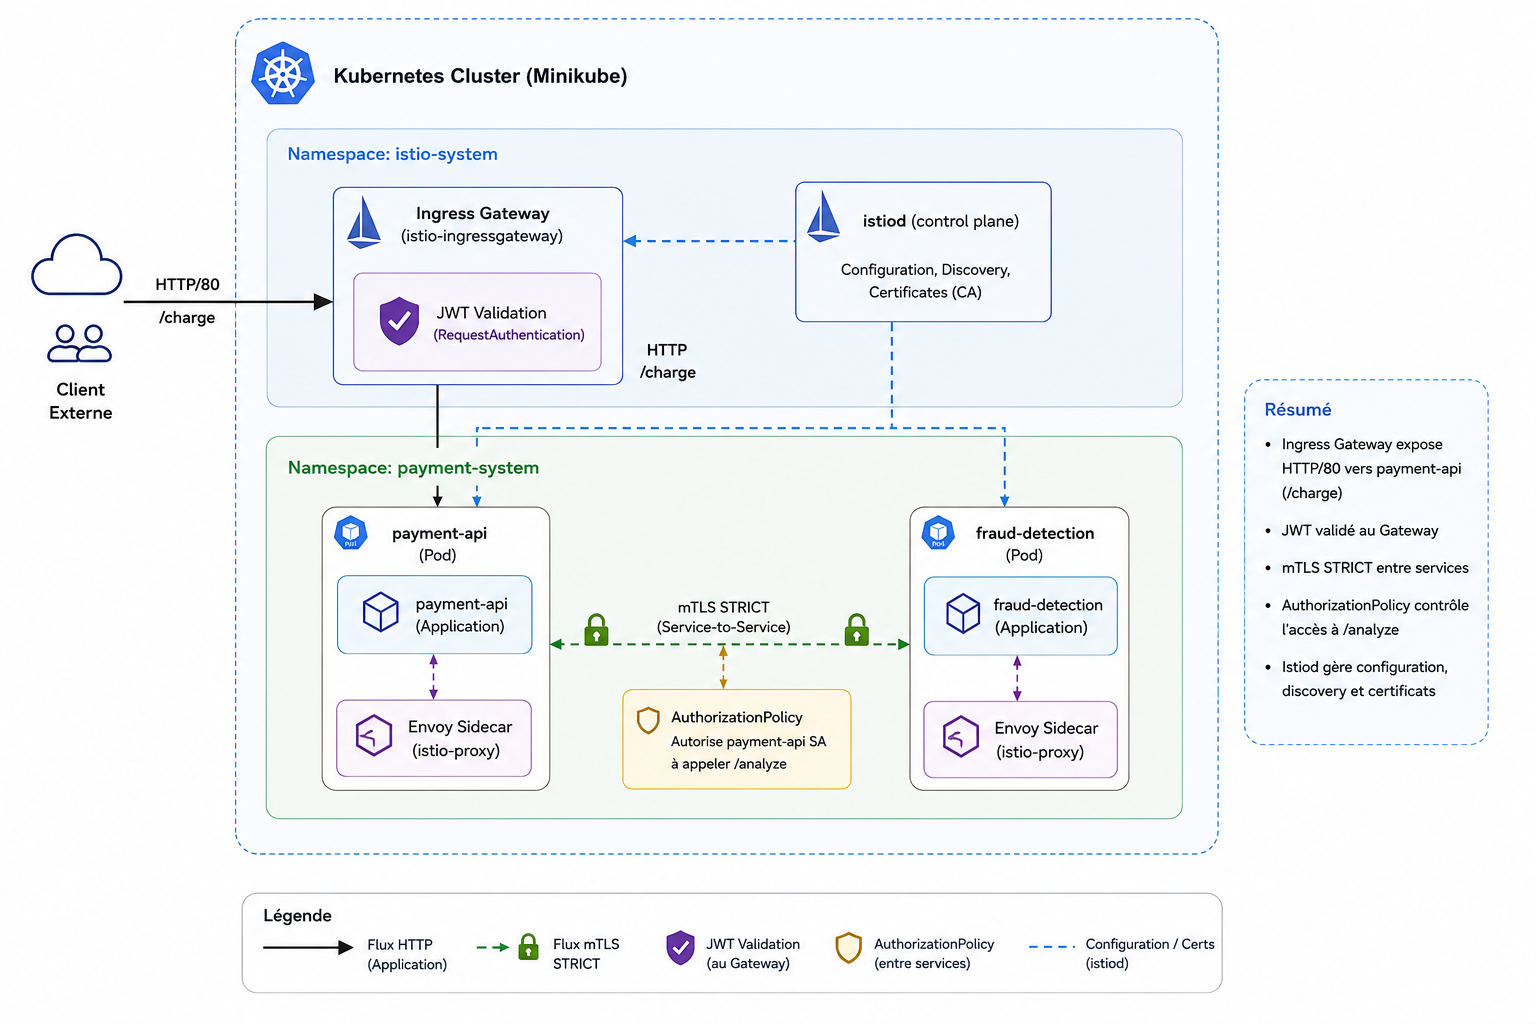
\includegraphics[width=\textwidth]{chapitres/Archi k8s avec Istio.png}
  \caption{Architecture du prototype Service Mesh --- Kubernetes/Minikube avec Istio.}
  \label{fig:architecture_prototype}
\end{figure}

\subsection{Les Deux Microservices}

Le système comprend deux microservices métier aux rôles complémentaires~[16] :

\begin{itemize}[topsep=4pt, itemsep=3pt]
  \item \textbf{Payment-API (Go, port 8080) :} service principal exposé via
        l'Ingress Gateway~[1]. Il expose les endpoints \texttt{/health},
        \texttt{/ready} et \texttt{/charge}, traite les requêtes de paiement et
        délègue l'analyse de risque à \texttt{fraud-detection} via un appel
        mTLS~[9]. Il s'exécute sous le ServiceAccount \texttt{payment-api} avec
        100m CPU et 128Mi RAM.

  \item \textbf{Fraud-Detection (Python/Flask, port 8080) :} service interne
        d'analyse de risque. Il expose les endpoints \texttt{/health},
        \texttt{/ready} et \texttt{/analyze}, et n'est accessible que depuis
        \texttt{payment-api} via validation SPIFFE~[7]. Il s'exécute sous le
        ServiceAccount \texttt{fraud-detection} avec les mêmes ressources
        allouées.
\end{itemize}

\subsection{Ressources de Configuration Istio et Kubernetes}

L'architecture de sécurité et de routage repose sur huit ressources de
configuration déployées dans le répertoire \texttt{mesh-config/}, réparties
entre les CRDs Istio gérés par \texttt{istiod} et une ressource Kubernetes
native opérant au niveau CNI~[11].

\subsubsection*{Istio CRDs (gérés par istiod)}

\begin{itemize}[topsep=4pt, itemsep=6pt]

  \item \textbf{VirtualServices (3) :} règles de routage avec retry automatique
        ($3\times$, \texttt{perTryTimeout=10s}) et timeout global de 30 secondes
        par appel inter-service~[1]. Deux VirtualServices couvrent le trafic
        interne (\texttt{payment-api}, \texttt{fraud-detection}) ; un troisième
        gère le trafic entrant depuis le Gateway.

  \item \textbf{DestinationRules (2) :} politique de trafic pour
        \texttt{payment-api} et \texttt{fraud-detection} : load balancing
        round-robin, connection pool limité à 100 connexions simultanées
        (\texttt{maxRequestsPerConnection=2}), et outlier detection qui éjecte
        un hôte après 5 erreurs 5xx consécutives (fenêtre de 30 secondes,
        durée d'éjection de 30 secondes)~[1,8].

  \item \textbf{Gateway (1) :} point d'entrée externe exposé sur le port 80 en
        HTTP~[1]. \textbf{Limitation : aucune terminaison TLS n'est configurée}
        --- le trafic entre le client et le gateway transite en clair. Un
        déploiement en production requiert l'ajout d'un certificat et le passage
        en HTTPS/443~[9].

  \item \textbf{PeerAuthentication (1) :} enforce mTLS \texttt{STRICT} sur tous
        les pods du namespace \texttt{payment-system}~[9,1]. Les certificats sont
        émis et renouvelés automatiquement par \texttt{istiod}. Tout client sans
        sidecar ou certificat valide est rejeté au niveau du proxy Envoy.

  \item \textbf{RequestAuthentication (1) :} valide les tokens JWT (RS256) sur
        \texttt{payment-api}~[1]. Issuer attendu : \texttt{https://testing.com},
        audience : \texttt{payment-api}, avec \texttt{forwardOriginalToken=true}
        afin que les services en aval reçoivent le token original. La clé de
        vérification est fournie via un JWKS inline --- adapté à un environnement
        de démonstration ; un endpoint JWKS distant doit être utilisé en
        production.

  \item \textbf{AuthorizationPolicies (2) :} contrôle d'accès zero-trust à
        granularité fine~[5] :
        \begin{itemize}[topsep=2pt, itemsep=2pt]
          \item \texttt{payment-api} : \texttt{/health} et \texttt{/ready} sont
                accessibles sans restriction (sondes liveness/readiness) ;
                \texttt{POST /charge} est autorisé uniquement depuis le namespace
                \texttt{istio-system} avec le claim JWT \texttt{role=customer},
                ou depuis le service account
                \texttt{cluster.local/ns/payment-system/sa/fraud-detection}.
          \item \texttt{fraud-detection} : \texttt{POST /analyze},
                \texttt{/health} et \texttt{/ready} sont autorisés uniquement
                depuis le service account
                \texttt{cluster.local/ns/payment-system/sa/payment-api}. Tout
                autre accès est refusé par défaut~[5].
        \end{itemize}

  \item \textbf{EnvoyFilter (1) :} rate limiting local appliqué directement sur
        \texttt{istio-ingressgateway}, en amont de tout routage~[8]. Token bucket
        : 20 tokens par seconde, rechargé toutes les secondes
        (\texttt{fill\_interval=1s}), appliqué à 100\,\% des requêtes. Cette
        limite est locale à chaque replica du gateway --- elle ne constitue pas
        un rate limiting distribué global.

\end{itemize}

\subsubsection*{Ressource Kubernetes native}

\begin{itemize}[topsep=4pt, itemsep=3pt]
  \item \textbf{NetworkPolicies (2)~[12] :} isolation réseau au niveau du CNI,
        indépendante du Service Mesh Istio. Cette couche reste effective même en
        cas d'absence ou de mauvaise configuration des sidecars, assurant une
        défense en profondeur~[5]. Les règles imposent :
        \begin{itemize}[topsep=2pt, itemsep=2pt]
          \item \textbf{Ingress :} seules les communications provenant du
                namespace \texttt{payment-system} (label
                \texttt{name=payment-system}) sont autorisées sur le port TCP
                8080.
          \item \textbf{Egress :} les sorties réseau sont limitées au namespace
                \texttt{payment-system} et au service DNS du cluster
                (\texttt{kube-dns}, port UDP 53).
        \end{itemize}
\end{itemize}

\subsection{Flux de Requête et Gestion des Certificats}

Le flux complet d'une requête de paiement traverse les étapes suivantes : le
client envoie une requête HTTP \texttt{/charge} à l'Ingress Gateway (port 31629),
qui vérifie l'autorisation et route vers \texttt{payment-api}~[1]. Le sidecar
Envoy intercepte la requête, applique les règles du VirtualService, puis initie
un handshake mTLS TLS~1.3 vers \texttt{fraud-detection}~[9]. Les certificats
mutuels sont vérifiés via leur identité SPIFFE~[7] et la réponse est renvoyée
chiffrée dans le même tunnel mTLS. Ce déroulement est illustré par la
figure~\ref{fig:flux_requete}.

\begin{figure}[H]
  \centering
  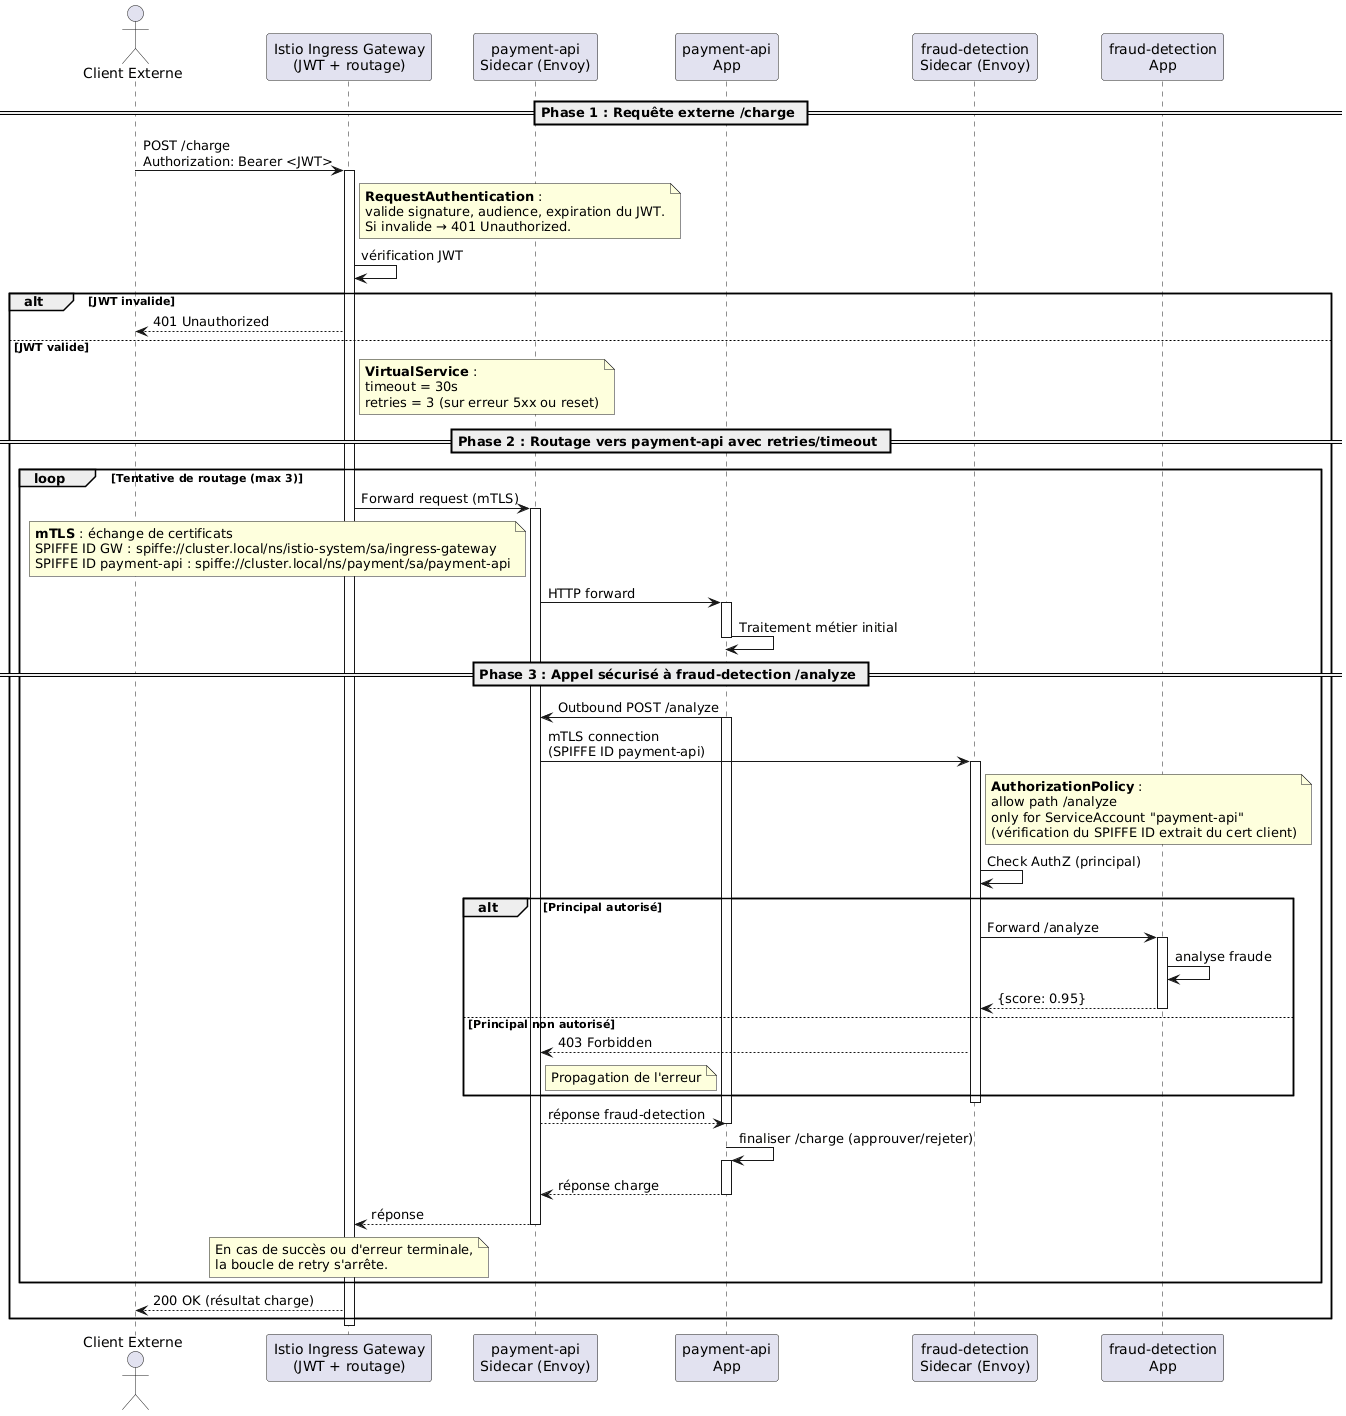
\includegraphics[width=\textwidth]{chapitres/flux.png}
  \caption{Diagramme de séquence : flux complet d'une requête \texttt{/charge}
    en trois phases.}
  \label{fig:flux_requete}
\end{figure}

Les certificats X.509 sont émis par l'autorité de certification Istio avec
l'identité SPIFFE
\texttt{spiffe://cluster.local/ns/payment-system/sa/\{service\}}~[7], stockés dans\linebreak
\texttt{/var/run/secrets/workload-spiffe/} et renouvelés automatiquement toutes
les 24 heures sans redémarrage de pod~[9]. Le \textit{Perfect Forward Secrecy}
(PFS) est activé, garantissant que la compromission d'une clé ne compromet pas
les sessions passées. Le processus complet de génération, de distribution et de
rotation des certificats est illustré par la figure~\ref{fig:cycle_certificats}.

\begin{figure}[H]
  \centering
  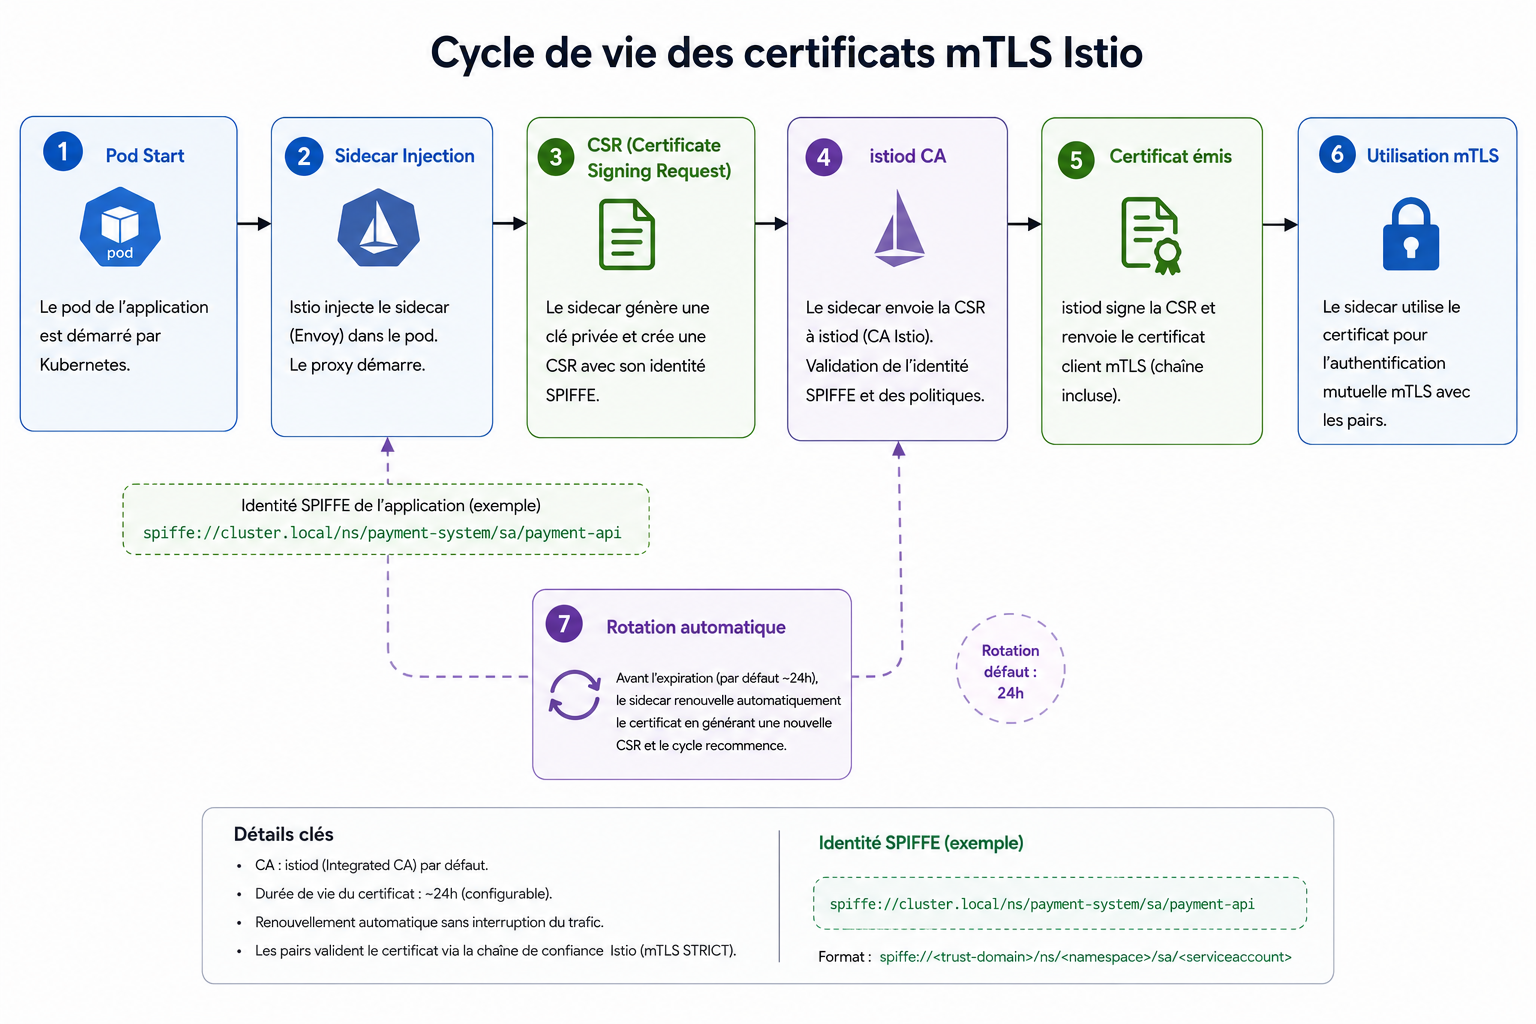
\includegraphics[width=\textwidth]{chapitres/Cycle de vie mTLS cert.png}
  \caption{Cycle de vie des certificats mTLS Istio.}
  \label{fig:cycle_certificats}
\end{figure}

% ─────────────────────────────────────────────────────────────────────────────
\begin{samepage}
\section*{Conclusion}
% ─────────────────────────────────────────────────────────────────────────────

Ce chapitre a présenté le Service Mesh comme une réponse architecturale aux
défis de sécurité posés par les microservices~[16]. Nous avons introduit le concept
et sa structuration en Data Plane et Control Plane~[1,8], détaillé les composants
déployés dans Istio et justifié son choix face aux solutions concurrentes.
L'architecture du prototype --- deux microservices sur Kubernetes avec huit
ressources de configuration Istio et Kubernetes~[11,12] --- constitue la base
concrète sur laquelle s'appuient les analyses des chapitres suivants.
\end{samepage}